\documentclass[10pt]{article}

\usepackage[T1]{fontenc}
\usepackage{geometry}
\usepackage{amsmath, amssymb, amsthm}
\usepackage{bm}
\usepackage{cancel}
\usepackage{xcolor}
\usepackage{graphicx}
\usepackage{caption}
\usepackage{subcaption}
\usepackage{hyperref}
\usepackage{float}

\title{Mathematical Methods II - Assignment X}
\author{Satvik Saha}
\date{}

\geometry{a4paper, margin=1in}
\setlength\parindent{0pt}
\renewcommand{\labelenumi}{(\alph{enumi})}
\renewcommand\CancelColor{\color{red}}
% \renewcommand\qedsymbol{$\blacksquare$}
\newcommand\var[1]{\operatorname{Var}(#1)}
\newcommand\E[1]{\operatorname{E}[#1]}

\begin{document}
        \par\textbf{IISER Kolkata} \hfill \textbf{Assignment X}
        \vspace{3pt}
        \hrule
        \vspace{3pt}
        \begin{center}
                \LARGE{\textbf{MA 2103 : Mathematical Methods II}}
        \end{center}
        \vspace{3pt}
        \hrule
        \vspace{3pt}
        Satvik Saha, \texttt{19MS154}\hfill\today
        \vspace{20pt}

        A set of $n$ data points $(x_i, y_i)$ can be fitted to the linear curve $y = mx + c$, where the regression coefficients $m$ and $c$
        are given by
        \[
                m = \frac{\sigma_{xy}}{\sigma_{x}^2} = \frac{n\sum xy - \sum x\sum y}{n\sum x^2 - (\sum x)^2}, \qquad
                c = \overline{y} - m\overline{x} = \frac{\sum y - m\sum{x}}{n}.
        \]
        Note that $\sigma_{xy}$ is the covariance between $x$ and $y$, given by $\E{(x - \overline{x})(y - \overline{y})}$.
        Also, $\sigma_x^2 = \sigma_{xx}$ is the variance of $x$, given by $\E{(x - \overline{x})^2}$.
        The Pearson correlation coefficient $r_{xy}$ is calculated as
        \[
                r_{xy} = \frac{\sigma_{xy}}{\sigma_x\sigma_y} 
                        = \frac{n\sum xy - \sum x\sum y}{\sqrt{n\sum x^2 - (\sum x)^2}\sqrt{n\sum y^2 - (\sum y)^2}}.
        \]
        Thus, all we need to calculate are $\sum x$, $\sum y$, $\sum x^2$, $\sum y^2$ and $\sum xy$.
        The 95\% confidence interval of the predicted quantity $y$ is given by $y \pm 1.96 \sigma /\sqrt{n}$.

        \paragraph{Problem 1.} When an anthropologist finds skeletal remains, they need to figure out the height of the person.
        The height of a person (in cm) and the length of their metacarpal bone 1 (in cm) are given. Create a scatter plot and
        find a regression equation between the height of a person and the length of their metacarpal. Then use the regression equation to
        find the height of a person for a metacarpal length of 44 cm and for a metacarpal length of 55 cm.
        Which height that you calculated do you think is closer to the true height of the person? Why? \\

        \textit{Solution.} 
        We have $n = 9$. We calculate 
        \[
                \sum x = 409, \qquad \sum y = 1545, \qquad \sum x^2 = 18707, \qquad \sum y^2 = 265699, \qquad \sum xy = 70416.
        \]
        Thus, we further calculate
        \[
                m = 1.700, \qquad c = 94.428, \qquad r_{xy} = 0.856.
        \]
        The correlation is very strong.
        \begin{figure}[H]
        \centering
        \begin{subfigure}[b]{0.49\textwidth}
                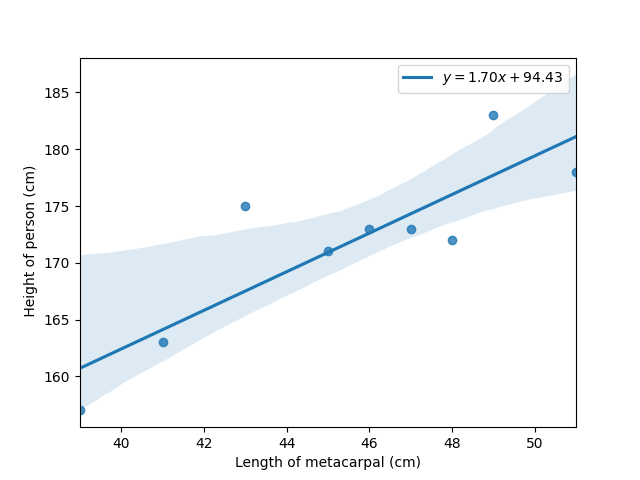
\includegraphics[width=\textwidth]{./10_1_1.png}
        \end{subfigure}
        \begin{subfigure}[b]{0.49\textwidth}
                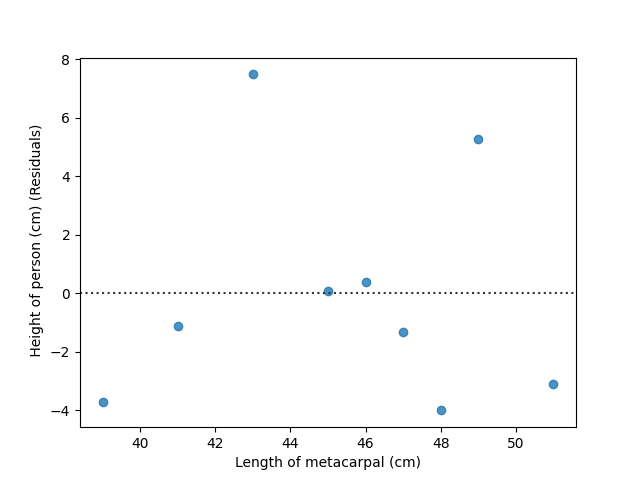
\includegraphics[width=\textwidth]{./10_1_2.png}
        \end{subfigure}
        \caption{Scatter plot of the data and the linear regression curve, with the 95\% confidence interval shaded in.
        The residuals are shown on the right.}
        \label{fig:metacarpal}
        \end{figure}

        Using our regression equation, we predict that a metacarpal length of 44 cm corresponds to a height of 169.2 cm,
        and that a metacarpal length of 55cm corresponds to a height of 187.9 cm.
        We have more confidence in the first prediction since 44 cm lies within the range of the data, so we are interpolating.
        In contrast, the values of 55cm lies outside the range, so we are extrapolating. The linear trend we have predicted may not remain valid
        beyond the range of data supplied, and we can make very little judgement without additional data.

        \paragraph{Problem 2.} The given table contains the value of a house and the amount of rental income in a year that the house brings in.
        Create a scatter plot and find a regression equation between house value and rental income. Then use the regression equation to find
        the rental income for a house worth \$230,000, then for a house worth \$400,000. 
        Which rental income that you calculated do you think is closer to the true rental income? Why? \\
        
        \textit{Solution.} 
        We have $n = 48$. We calculate 
        \[
                \sum x = 8370000, \qquad \sum y = 461344,
        \]\[
                \sum x^2 = 1686454500000, \qquad \sum y^2 = 4664378368, \qquad \sum xy = 85974616000.
        \]
        Thus, we further calculate
        \[
                m = 0.024, \qquad c = 5364, \qquad r_{xy} = 0.765.
        \]
        The correlation is strong.
        \begin{figure}[H]
        \centering
        \begin{subfigure}[b]{0.49\textwidth}
                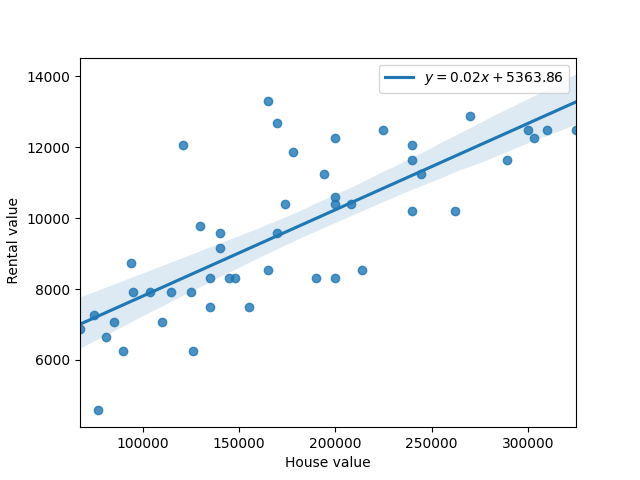
\includegraphics[width=\textwidth]{./10_2_1.png}
        \end{subfigure}
        \begin{subfigure}[b]{0.49\textwidth}
                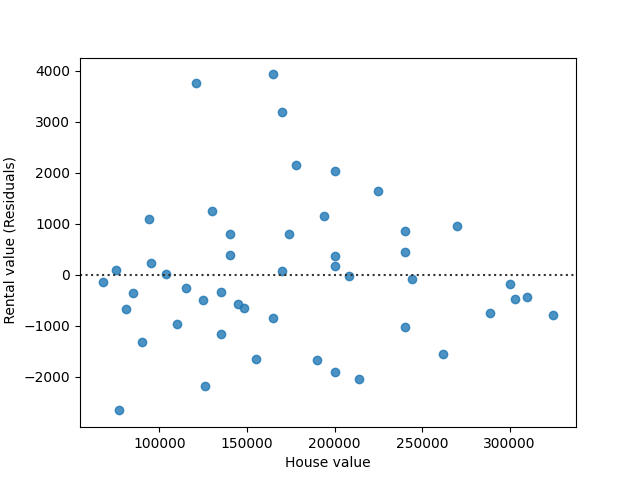
\includegraphics[width=\textwidth]{./10_2_2.png}
        \end{subfigure}
        \caption{Scatter plot of the data and the linear regression curve, with the 95\% confidence interval shaded in.
        The residuals are shown on the right.}
        \label{fig:rental}
        \end{figure}

        Using our regression equation, we predict that a house value of \$230,000 corresponds to a rental value of \$10,966,
        and that \$400,000 corresponds to \$15107.
        We have more confidence in the first prediction than in the second for the same reasons as in before; \$230,000 lies
        within the range of data but \$400,000 does not. Thus, we are interpolating in the first case while extrapolating in the second.

        \paragraph{Problem 3.} The World Bank collects information on the life expectancy of a person in each country and the fertility rate
        per woman in the country. The data for 24 randomly selected countries in 2011 have been given. Create a scatter plot of the data
        and find a linear regression equation between fertility rate and life expectancy. Then use the regression equation to find the life
        expectancy for a country that has a fertility rate of 2.7, and for a country with fertility rate of 8.1.
        Which life expectancy which you calculated do you think is closer to the true life expectancy? Why?\\
        
        \textit{Solution.} 
        We have $n = 24$. We calculate 
        \[
                \sum x = 72.5, \qquad \sum y = 1695.8, \qquad \sum x^2 = 285.71, \qquad \sum y^2 = 121525, \qquad \sum xy = 4808.87.
        \]
        Thus, we further calculate
        \[
                m = -4.706, \qquad c = 84.873, \qquad r_{xy} = -0.931.
        \]
        The anti-correlation is very strong.
        \begin{figure}[H]
        \centering
        \begin{subfigure}[b]{0.49\textwidth}
                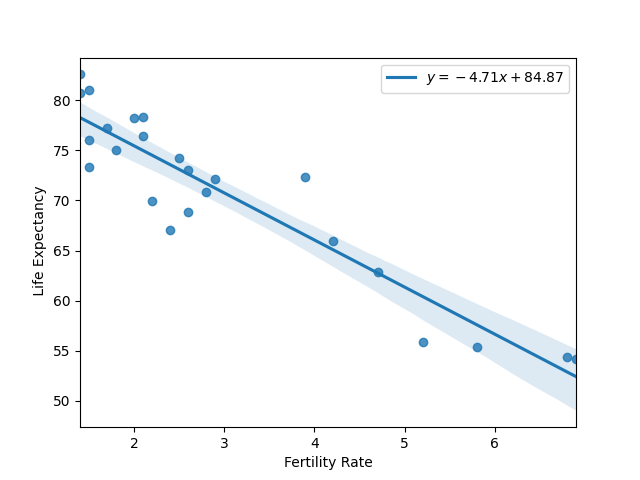
\includegraphics[width=\textwidth]{./10_3_1.png}
        \end{subfigure}
        \begin{subfigure}[b]{0.49\textwidth}
                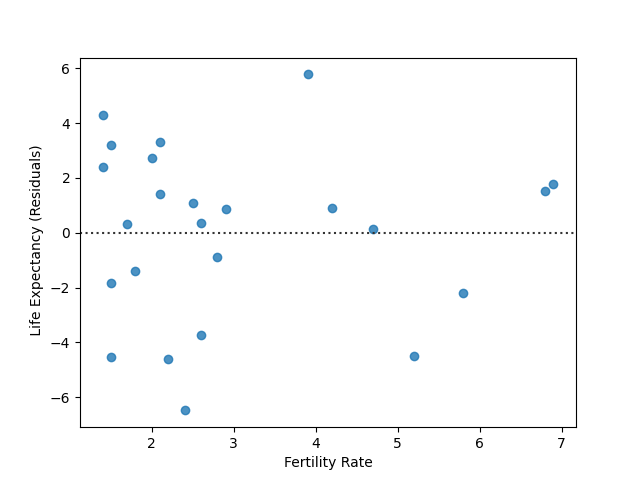
\includegraphics[width=\textwidth]{./10_3_2.png}
        \end{subfigure}
        \caption{Scatter plot of the data and the linear regression curve, with the 95\% confidence interval shaded in.
        The residuals are shown on the right.}
        \label{fig:expectancy}
        \end{figure}

        Using our regression equation, we predict that a fertility rate of 2.7 corresponds to a life expectancy of 72.2 years,
        and that 8.1 corresponds to 46.8 years.
        Again, we have more confidence in the first prediction than in the second since we are interpolating in the first case, extrapolating 
        in the second.

        \paragraph{Problem 4.} Different species have different body weights and brain weights as given.
        Create a scatter plot and find a regression equation between body weights and brain weights. Then use the regression equation to 
        find the brain weight for a species that has a body weight of 62 kg and for a species that has a body weight of 180,000 kg.
        Which brain weight that you calculated do you think is closer to the true brain weight? Why?\\

        \textit{Solution.} 
        We have $n = 27$. We calculate 
        \[
                \sum x = 44759.15, \qquad \sum y = 22.84,
        \]\[
                \sum x^2 = 1249124518.5625, \qquad \sum y^2 = 104.6602, \qquad \sum xy = 303854.731.
        \]
        Thus, we further calculate
        \[
                m = 0.000226, \qquad c = 0.471, \qquad r_{xy} = 0.840.
        \]
        The correlation appears to be very strong.
        \begin{figure}[H]
        \centering
        \begin{subfigure}[b]{0.49\textwidth}
                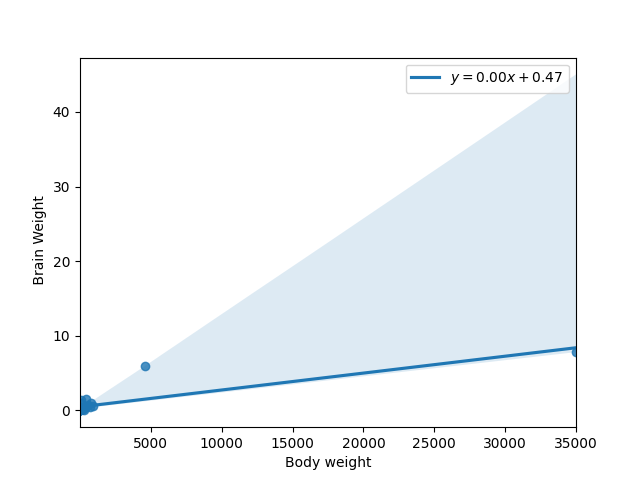
\includegraphics[width=\textwidth]{./10_4_1.png}
        \end{subfigure}
        \begin{subfigure}[b]{0.49\textwidth}
                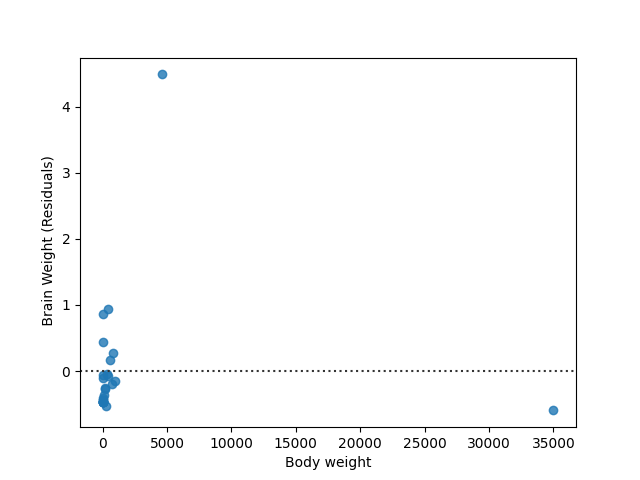
\includegraphics[width=\textwidth]{./10_4_2.png}
        \end{subfigure}
        \caption{Scatter plot of the data and the linear regression curve, with the 95\% confidence interval shaded in.
        The residuals are shown on the right.}
        \label{fig:brain}
        \end{figure}

        It is clear that the data as it stands is not suitable for linear regression, due to the presence of the two outliers far above and beyond 
        1000 kg. These significantly bias the regression parameters, acting as a `high leverage point'.
        
        Upon removing the outliers, we have $n = 25$, so
        \[
                \sum x = 5159.15, \qquad \sum y = 9.04,
        \]\[
                \sum x^2 = 2964518.5625, \qquad \sum y^2 = 7.82, \qquad \sum xy = 3254.731.
        \]
        Thus,
        \[
                m = 0.000731, \qquad c = 0.212, \qquad r_{xy} = 0.472.
        \]
        This means that the correlation is moderate.
        \begin{figure}[H]
        \centering
        \begin{subfigure}[b]{0.49\textwidth}
                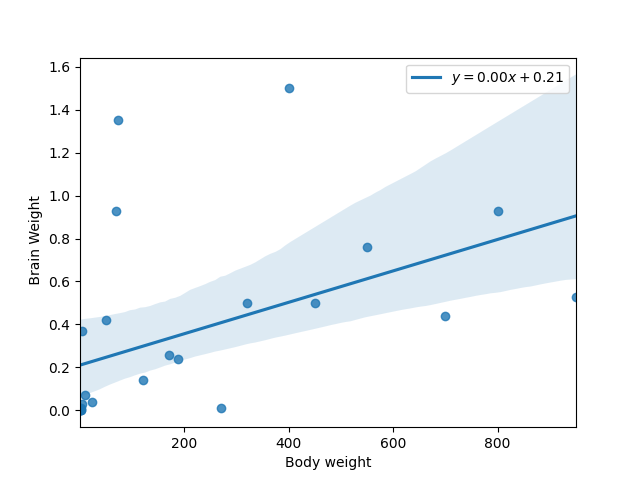
\includegraphics[width=\textwidth]{./10_4_1x.png}
        \end{subfigure}
        \begin{subfigure}[b]{0.49\textwidth}
                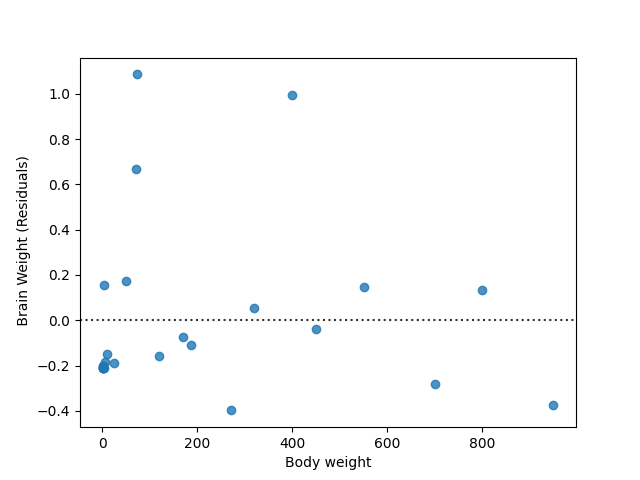
\includegraphics[width=\textwidth]{./10_4_2x.png}
        \end{subfigure}
        \caption{Scatter plot of the cleaned data and the linear regression curve, with the 95\% confidence interval shaded in.
        The residuals are shown on the right.}
        \label{fig:brain_clean}
        \end{figure}
        Now, it is clear that there is far less correlation between the two data then we were lead to believe from the previous calculation.

        Using the repression equation, we predict that a body weight of 62 kg corresponds to a brain weight of 0.256 kg, and that
        180,000 kg corresponds to 131.8 kg.
        Again, we have far more confidence in the first prediction than in the second since we are interpolating in the first case, extrapolating 
        in the second.
        We have very little confidence in either prediction to begin with, due to the moderate correlation between the two data. \\

        Anscombe's quartet gives examples of datasets with identical regression and statistical parameters, yet only the first is suitable for
        linear regression.

        \paragraph{Problem 5.} For the given grouped data of 50 Grade 10 girls, find out the mean, median and mode.
        \begin{table}[H]
                \centering
                \label{tab:grouped}
                \begin{tabular}{cccc}\hline
                Height (cm)     & Midpoint $x$ (cm)     & Frequency $f$ & Cumulative frequency  \\\hline
                150-155         & 152.5                 & 4             & 4 \\
                155-160         & 157.5                 & 7             & 11 \\
                160-165         & 162.5                 & 18            & 29 \\
                165-170         & 167.5                 & 11            & 40 \\
                170-175         & 172.5                 & 6             & 46 \\
                175-180         & 177.5                 & 4             & 50 \\\hline
                \end{tabular}
        \end{table}

        \textit{Solution.} Note that the class intervals exclude the upper value, so the midpoints are calculated accordingly.

        The mean is calculated as
        \[
                \text{Mean} = \frac{1}{n}\sum f_i x_i = 164.5.
        \]
        We identify the median class as the 160-165 one, since the cumulative frequency of $25$ lies within it. We now calculate the
        median as
        \begin{align*}
                \text{Median} &= \text{(lower class boundary of median group)} 
                        + \frac{n/2 - (\text{cumulative frequency of prior groups})}{\text{(frequency of median group)}}\times
                        \text{(width)}  \\
                        &= 160 + \frac{25 - 11}{18}\cdot 5 \\
                        &= 163.89.
        \end{align*}

        The modal group is also the 160-165 one, since its frequency of 18 is the highest. Setting this frequency to $f_m$, we calculate
        \begin{align*}
                \text{Mode} &= \text{(lower class boundary of modal group)} + \frac{f_m - f_{m - 1}}{(f_m - f_{m - 1}) + (f_m - f_{m + 1})} 
                        \times\text{(width)} \\
                        &= 160 + \frac{18 - 7}{(18 - 7) + (18 - 11)}\cdot 5 \\
                        &= 163.06.
        \end{align*}
\end{document}
